\documentclass{beamer}
\usepackage{geometry, amsfonts, amsmath, tikz, multicol, tikz-imagelabels, 
            multirow, pifont, xcolor, tcolorbox}

\usetheme{Madrid}
\usecolortheme{cormorant}
\title [UVA Seminar]{Search for a Self Interacting Dark Mater at the CMS Experiment }
\author[Maria Jose]{Maria Jose}
\date{\today}
\institute[UVA]{University of Virginia}
\hypersetup{
    colorlinks=true,
    linkcolor=cyan,
    filecolor=magenta,      
    urlcolor=cyan,
    pdftitle={Overleaf Example},
    pdfpagemode=FullScreen,
    }

\definecolor{uvablue}{RGB}{35,45,75}
\definecolor{uvaorange}{RGB}{229,114,0}
\definecolor{UniBlue}{RGB}{83,121,170}
\definecolor{forestgreen}{RGB}{0,128,0}
\definecolor{bronze}{rgb}{0.8, 0.5, 0.2}
\definecolor{purple}{RGB}{128,0,128}
\definecolor{maroon}{RGB}{184,15,10}
\definecolor{grey}{RGB}{128,128,128}
\definecolor{bondiblue}{rgb}{0.0, 0.58, 0.71}
\definecolor{gold}{RGB}{160,116,10}
\definecolor{peacockblue}{RGB}{0,164,180}

%\setbeamercolor{frame}{bg=black, fg =white}
%\setbeamercolor{frametitle right}{bg=gray!60!white}
%setbeamercolor{palette primary}{bg=black,fg=white}
\setbeamercolor{structure}{fg=uvaorange}
\setbeamercolor*{frametitle}{ fg =peacockblue}
\setbeamercolor*{title}{ fg = cyan}
%\setbeamercolor{alerted text}{fg=red!85!black}
\setbeamercolor*{palette primary}{fg =peacockblue}
\setbeamercolor*{palette secondary}{fg =peacockblue}
\setbeamercolor*{palette tertiary}{fg =peacockblue}
\setbeamercolor*{palette quaternary}{fg =peacockblue }
%\setbeamercolor*{background canvas}{bg=uvablue}
%


%\setbeamercolor*{block body}{fg=black,bg=black!10}
%\setbeamercolor*{block title alerted}{,bg=black!15}
%\setbeamercolor*{block title example}{parent(0,164,180)=example text,bg=black!15}

\imagelabelset{
coordinate label font = \sffamily\bfseries\tiny,
coordinate label distance = 1mm,
coordinate label back = white ,
coordinate label text = uvaorange,
annotation font = \normalfont\tiny,
}
%\logo{%
%  
% % 
\includegraphics[width=1cm,height=1cm,keepaspectratio]{CMSlogo.png}%
%   \hspace{\dimexpr\paperwidth -1.5cm}%
%  \vspace{\dimexpr\paperwidth }%
%  \includegraphics[width=1cm,height=1cm,keepaspectratio]{images.png}%
% 
%}

\begin{document}

\maketitle
\begin{frame}[t]{\textbf{Self Interacting Dark Matter Model}}
    \begin{columns}
    \begin{column}{.25\textwidth}
    \centering
    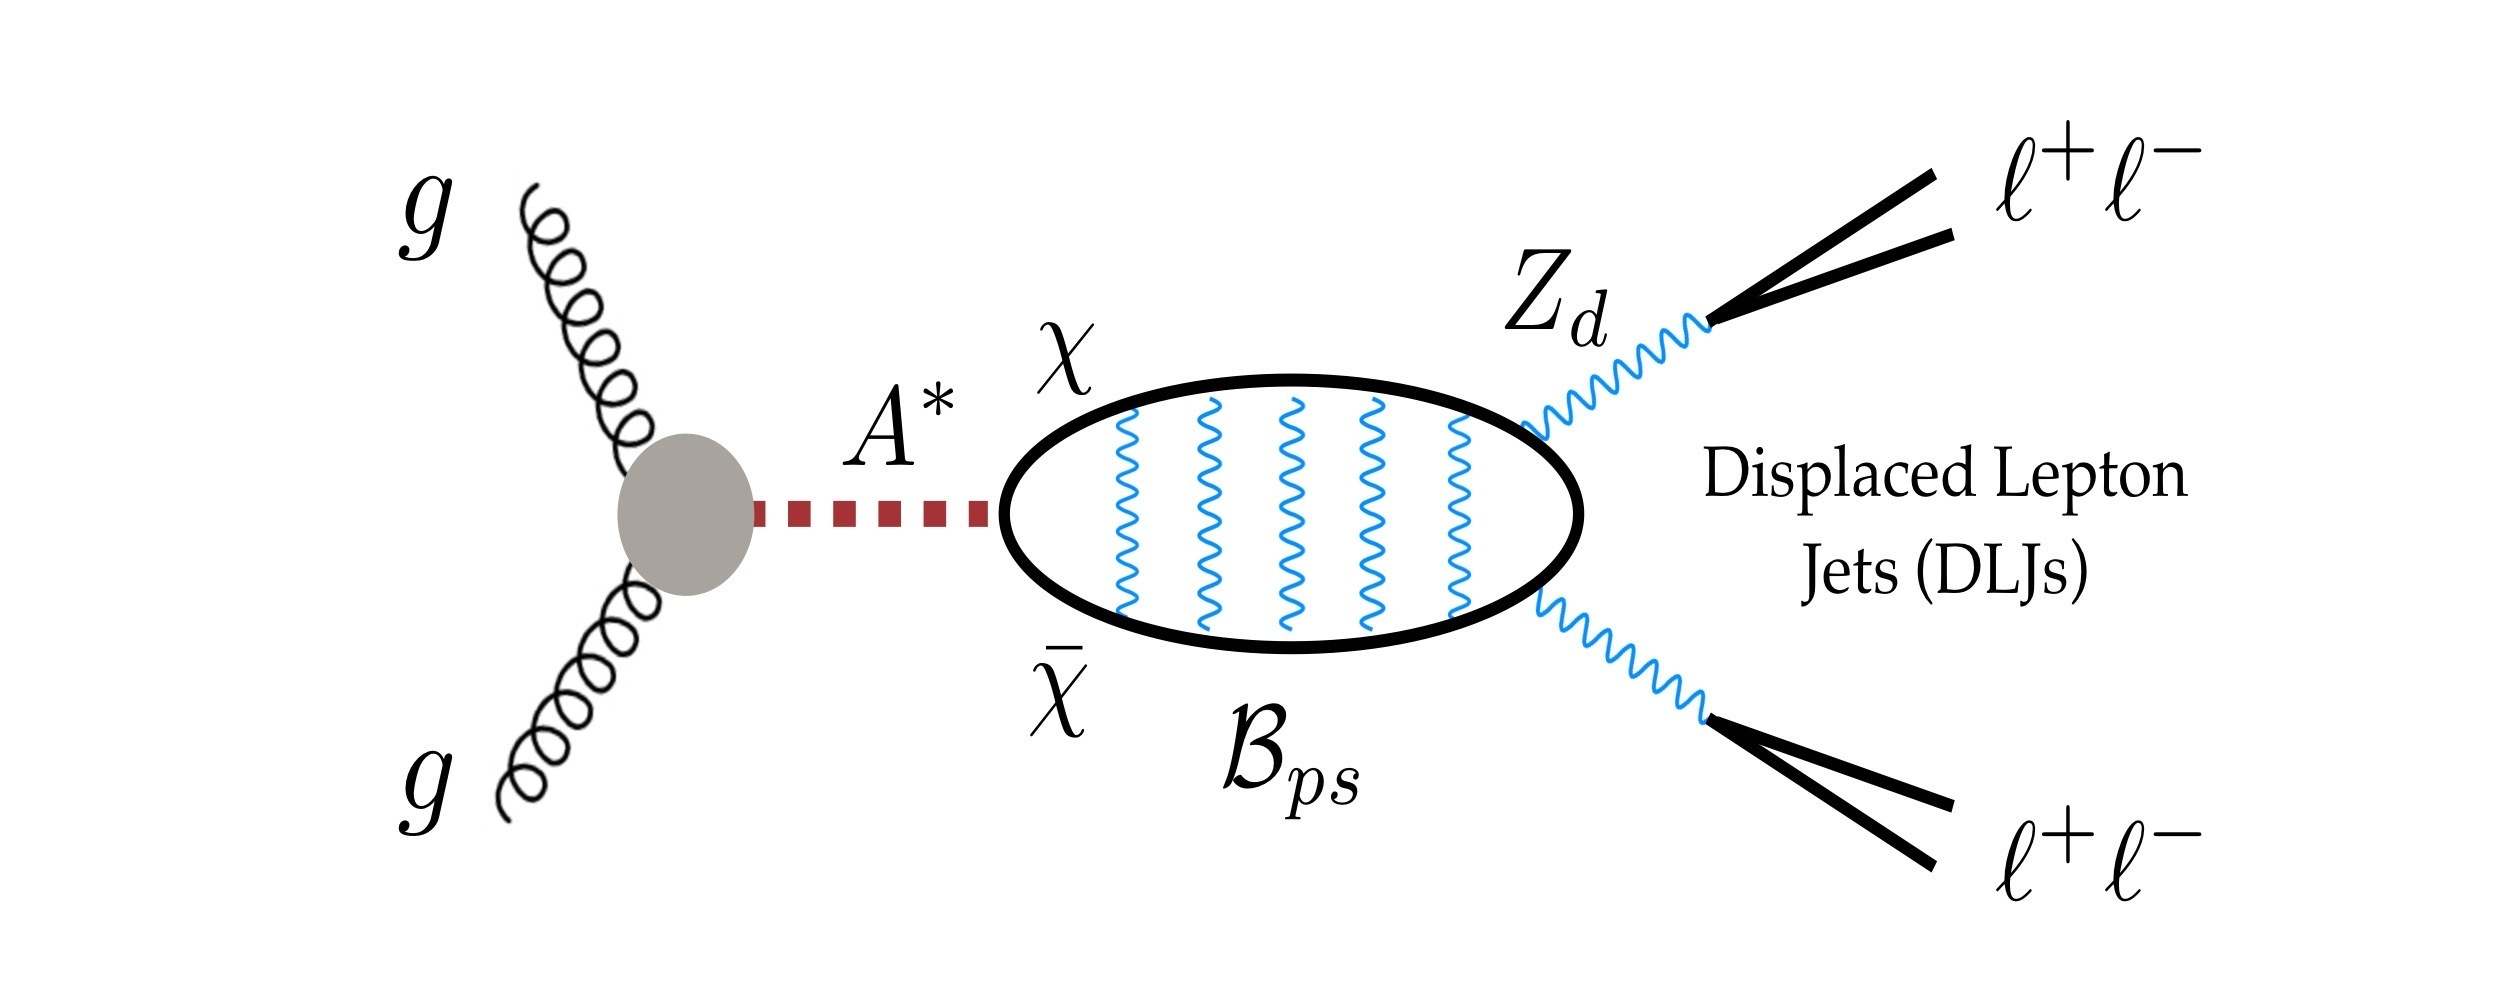
\includegraphics[width =3cm, height = 2.5 cm]{../sidm_intro_files/FeyDia.jpg}
    \end{column}
    \begin{column}{.5\textwidth}
    \begin{enumerate}
        \item Light \textbf{$Z_d$} $\rightarrow$ \textcolor{peacockblue}{Boosted $Z_d$}
           \item Small $Z_d$ - SM Coupling \\ $\rightarrow$ \textcolor{peacockblue}{Long-Lived $Z_d$}
    \end{enumerate}
    \begin{tcolorbox}[colback=black,
                      colframe=uvaorange, coltext = white]
    
            Displaced decays of boosted $Z_d$ $\rightarrow$ \textcolor{peacockblue}{Displaced, collimated leptons }(\textcolor{uvaorange}{Displaced Lepton Jets (LJs)})
    \end{tcolorbox}
        
    \end{column}
    \begin{column}{.25\textwidth}
    \centering
    \begin{annotationimage}{width=3cm, height=2.5cm}{../sidm_intro_files/lj.png}
    %\draw[coordinate label  = {$Z_d \rightarrow ee$ at (0.5, -.05)}];
    \draw[coordinate label  = {\textcolor{bondiblue}{LJ}  at (0.5, 0.1)}];
    \draw[coordinate label  = {\textcolor{maroon}{$\mu/e$}  at (0.88, 0.9)}];
    \draw[coordinate label  = {\textcolor{maroon}{$\mu/e$}  at (0.61, 0.9)}];
    \end{annotationimage}
    \end{column}
    
    \end{columns}
    \begin{columns}
    \begin{column}{.4\textwidth}
    \centering
    \textbf{\textcolor{peacockblue}{Free Parameters:}}
    \begin{itemize}
         \item Bound state mass ($m_B$)
         \item Dark photon mass ($m_{Z_d}$)
         \item Kinetic mixing between $Z_d$ and SM, $\epsilon$
    \end{itemize}
        
    \end{column}
    
    \begin{column}{.3\textwidth}
    \centering
    \textbf{\textcolor{peacockblue}{Reconstruction \\
    Objects:}}
    \begin{itemize}
        \item PF electrons
         \item PF Photons
         \item PF Muons
         \item DSA Muons
    \end{itemize}
        
    \end{column}
    \begin{column}{.3\textwidth}
    \centering
    \textbf{\textcolor{peacockblue}{Signal:}}
    \begin{itemize}
        \item   $m_B$: from 100 to 1000 GeV.
         \item $m_{Z_d}$: from 0.25 to 5 GeV.
         \item $Z_d$ $L_{xy}$: from 0.3 to 300 cm.
    \end{itemize}
    \end{column}
    \end{columns}
    \end{frame}
    \begin{frame}{Dark Photon $p_T$}
        
    \end{frame}
    \begin{frame}
        \frametitle{Dark Photon $L_{xy}$}
    \end{frame}
    \begin{frame}
        \frametitle{$\Delta$R Between the Lepton Pairs}
    \end{frame}
\end{document}